\documentclass[final,hyperref={pdfpagelabels=false}]{beamer}
%%% THEME FOR THE POSTER %%%
\usetheme{LTS5}

%%% PACKAGES DECLARATION
%%%%%%%%%%%%%%%%%%%%%%%%%%%%%%%%%%%%%%%%%%%%%%%%%%%
% Signal Processing Laboratory (LTS5) - EPFL      %
% LaTeX beamposter template                       %
% Authors:                                        %
%   D. Perdios – dimitris.perdios@epfl.ch         %
%   A. Besson – adrien.besson@epfl.ch             %
% v0.1 - 08.05.17                                 %
% Typeset configuration: pdfLaTeX + Biber         %
%%%%%%%%%%%%%%%%%%%%%%%%%%%%%%%%%%%%%%%%%%%%%%%%%%%

% Poster related package
\usepackage[orientation=portrait,size=a0,scale=1.4]{beamerposter} % Use the beamerposter package for laying out the poster with a portrait orientation and an a0 paper size
\usepackage{textpos}

% Typesetting
\usepackage[T1]{fontenc}
\usepackage[utf8]{inputenc}
\usepackage[english]{babel}
\usepackage{lmodern} % latin modern font
\usepackage{exscale}
%\usepackage[scaled]{helvet} % sans serif typo
\usepackage{csquotes} % pro­vides ad­vanced fa­cil­i­ties for in­line and dis­play quo­ta­tions (better to load when using biblatex)
\usepackage{textcomp} % pro­vide many text sym­bols (such as baht, bul­let, copy­right, mu­si­cal­note, onequar­ter, sec­tion, and yen), in the TS1 en­cod­ing
%\usepackage{setspace}
%	\onehalfspacing % 1.5 linespaceing (already in CLS)
%\usepackage{fancyhdr} % pro­vides ex­ten­sive fa­cil­i­ties, both for con­struct­ing head­ers and foot­ers, and for con­trol­ling their use
\usepackage{siunitx} % SI units system typset
%\usepackage{enumitem}
%	\setlist[enumerate]{label*=\arabic*.,topsep=5pt,partopsep=0pt,parsep=0pt,itemsep=2pt}
%	\setlist[itemize]{topsep=5pt,partopsep=0pt,parsep=0pt,itemsep=2pt}
\usepackage{fontawesome} % high quality web icons

% Math
\usepackage{amsmath}
\usepackage{amsfonts}
\usepackage{amssymb}
\usepackage{amsthm}
\usepackage{bm}
\usepackage{mathdots}
%\usefonttheme[onlymath]{serif} % uncomment for serif math equations

% Figures
\usepackage{graphicx}
	\graphicspath{{figures/}}
\usepackage{xcolor}
\usepackage[font=small, labelfont=bf, format=plain, labelsep=space, figurename=Figure, tablename=Table]{caption}
\usepackage[labelfont=sf, labelformat=parens, labelsep=space]{subcaption}

% Tables
%\usepackage{multirow}
\usepackage{longtable} % use \linebreak instead of \\ in headers to avoid a bug with longtables (or longtabu) across two pages
\usepackage{booktabs} % the pack­age en­hances the qual­ity of ta­bles (toprule, bottomrule, etc.)
\usepackage{tabu}
%	\renewcommand{\arraystretch}{1.3}

% Codes
\usepackage{listings}
%	Some style definitions
\lstdefinestyle{lstLaTeX}{
	aboveskip=0pt,
	belowskip=0pt,
    language=[LaTeX]TeX,
    breaklines=true,
    basicstyle=\ttfamily\scriptsize,
%    keywordstyle=\color{blue},
%    identifierstyle=\color{magenta},
}
\lstdefinestyle{lstinlineLaTeX}{
	style=lstLaTeX, 		% uses the LaTeX listings style
    basicstyle=\ttfamily,	% only redefines the basicstyle
}
\lstdefinestyle{lstC}{
	aboveskip=0pt,
	belowskip=0pt,
	breaklines=true,
%	xleftmargin=\parindent,
	language=C,
	showstringspaces=false,
	basicstyle=\scriptsize\ttfamily,
	keywordstyle=\bfseries\color{green!40!black},
	commentstyle=\itshape\color{purple!40!black},
	identifierstyle=\color{blue},
	stringstyle=\color{orange},
}

% Algorithms
\usepackage{algorithm}
\usepackage{algpseudocode} % The algorithmicx package provides many possibilities to customize the layout of algorithms.
	\algrenewcommand\textproc{\small\MakeUppercase} %BEAMER ONLY: Latin Modern Sans fonts don't have small caps
%TODO: Check if can be put in .sty
	
% Others
\usepackage{beamerbasetheorems}
\usepackage{calc}
\usepackage{lipsum}
\usepackage{silence}
% Filter warnings issued by package biblatex starting with "Patching footnotes failed"
	\WarningFilter{biblatex}{Patching footnotes failed}

% Videos
%\usepackage[draft]{media9}
%\usepackage{media9}

% Emoji (thanks slide)
%\usepackage[nointegrals]{wasysym} % new characters (smiley)

% Biblatex
\usepackage[
	backend=biber,
	bibstyle=ieee,
	citestyle=ieee
]{biblatex} % style=ieee loads both, bibstyle and citestyle
\setbeamertemplate{bibliography item}[text]

% References and urls
% hyperref already loaded by beamer internally
\usepackage{url}
\usepackage{bookmark} % Im­ple­ments a new book­mark (out­line) or­ga­ni­za­tion for pack­age hy­per­ref
%%%%%%%%%%%%%%%%%%%%%%%%%%%%%%%%%%%%%%%%%%%%%%%%%%%
% Signal Processing Laboratory (LTS5) - EPFL      %
% LaTeX beamer template                           %
% Authors:                                        %
%   D. Perdios – dimitris.perdios@epfl.ch         %
%   A. Besson – adrien.besson@epfl.ch             %
% v0.1 - 18.11.16                                 %
% Typeset configuration: pdfLaTeX + Biber         %
%%%%%%%%%%%%%%%%%%%%%%%%%%%%%%%%%%%%%%%%%%%%%%%%%%%


% Specific package declarations
% *** TIKZ PACKAGES ***
\usepackage{xparse}
\usepackage{tikz}
\usetikzlibrary{shapes, arrows.meta, decorations.pathmorphing}
\usetikzlibrary{calc, positioning}
\usetikzlibrary{backgrounds}
\usetikzlibrary{intersections} % provides name path=
\usetikzlibrary{angles} % provides pic angle

\usepackage{etoolbox}

% Tikzset
\tikzset{%
	block/.style = {draw, shape=rectangle, thick, minimum height=2em, minimum width=2em},
	sum/.style = {draw, shape=circle, thick, inner sep=0pt},
	conn/.style={fill, shape=circle, minimum size=0.1cm, inner sep=0, outer sep=0},
	inout/.style={inner sep=0, outer sep=0},
	dot/.style={fill=, shape=circle, minimum size=\pgflinewidth, inner sep=0, outer sep=0},
	param/.style={inner sep=0, outer sep=1pt},
	loosely dotted round/.style={dash pattern=on 0pt off 6\pgflinewidth, line cap=round},
	%	transducer/.style = {shape=rectangle, draw=black, fill=black!20!white, thick, minimum height=0.15cm, minimum width=0.30cm, inner sep=0pt},
	%	my funny rectangle/.style n args={4}{%
	%    rectangle,
	%    draw,
	%    fit={(#1,#3) (#2,#4)}
	%%    append after command={\pgfextra{\let\mainnode=\tikzlastnode}
	%%      node[above right] at (\mainnode.north west) {#3}%
	%%      node[above left] at (\mainnode.north east) {#4}%
	%%      node[below left] at (\mainnode.north west) {#1}%
	%%      node[above left] at (\mainnode.south west) {#2}%
	%%    },
	%  }
}

%\def\td_number{3}

%\newcommand*{\transducer}[4][-1][-2]{\path[draw=black, fill=black!20!white] (#3, #1) rectangle (#4, #2)}

% arg1: lx (optional, default=1)
% arg2: ly (optional, default=2)
% arg3: x_center
% arg4: y_center
%\NewDocumentCommand{\transducer}{ O{-1} O{-2} m }{\path[draw=black, fill=black!20!white] (#3, #1) rectangle (#4, #2)}

\NewDocumentCommand{\rectangle}{ m m }{%
	%\newlength{\Xone}{#1 cm}%\pgfmathparse{#1+1}\pgfmathresult
	\path[draw=black, fill=black!20!white] #1 rectangle #2
}

%\pgfdeclarelayer{bg}    % declare background layer
%\pgfsetlayers{bg,main}  % set the order of the layers (main is the standard layer)

% This bascially automates a \newcommand{<name>}{} to ensure
% that a command with the given <name> does not already exist
\newcommand*{\pgfmathsetnewmacro}[2]{%
	\newcommand*{#1}{}% Error if already defined
	\pgfmathsetmacro{#1}{#2}%
}%

% Transducer commands
\newcommand*{\transducerNumb}{10}
\newcommand*{\transducerWidth}{0.75}
\newcommand*{\transducerHeight}{0.25}
\newcommand*{\transducerInitXPos}{3}
\newcommand*{\transducerXOffset}{1}
\definecolor{transducer-color}{gray}{0.8}
\newcommand*{\transducerLabeled}{9}

% Measurement commands
\newcommand*{\measurementLength}{6}
\definecolor{measurement-color}{gray}{0.7}

% Insonified domain
\pgfmathsetmacro{\domainXMin}{\transducerInitXPos}
\pgfmathsetmacro{\domainXMax}{12}
\pgfmathsetmacro{\domainZMin}{1}
\pgfmathsetmacro{\domainZLength}{7}
\pgfmathsetmacro{\domainZMax}{\domainZMin+\domainZLength}
\pgfmathsetmacro{\domainDxOffset}{1}
\pgfmathsetmacro{\domainDzOffset}{1}
\definecolor{domain-color}{gray}{0.7}
\definecolor{scatterer-color}{gray}{0}

% Wavefront and time of flight
\definecolor{wavefront-color}{gray}{0.5}

% Axes
\newcommand*{\axesOffset}{1.5}

% Conics
\definecolor{conic-color}{gray}{0}
% 	Ellipse
% http://tex.stackexchange.com/questions/75017/draw-an-ellipse-from-the-two-focus-points-foci-and-the-sum-of-the-distances-fr
\newcommand*{\ellipsebyfoci}[4]{% options (draw, fill, color, etc.), focus pt1, focus pt2, cste
	\path[#1] let \p1=(#2), \p2=(#3), \p3=($(\p1)!.5!(\p2)$)
	in \pgfextra{
		\pgfmathsetmacro{\angle}{atan2(\x2-\x1,\y2-\y1)}
		\pgfmathsetmacro{\distfoci}{veclen(\x2-\x1,\y2-\y1)/1cm} % convert back to cm
		\pgfmathsetmacro{\axeone}{#4/2}
		\pgfmathsetmacro{\axetwo}{sqrt(\axeone^2 - (0.5*\distfoci)^2)}
%		\pgfmathsetmacro{\focal}{veclen(\x2-\x1,\y2-\y1)/2/1cm}
%		\pgfmathsetmacro{\lentotcm}{\focal*2*#4}
%		\pgfmathsetmacro{\axeone}{(\lentotcm - 2 * \focal)/2+\focal}
%		\pgfmathsetmacro{\axetwo}{sqrt((\lentotcm/2)*(\lentotcm/2)-\focal*\focal}
	}
%	(\p3) ellipse[x radius=\axeone cm,y radius=\axetwo cm, rotate=\angle];
	(\p3) ellipse[x radius=\axeone,y radius=\axetwo, rotate={90-\angle}];
%	(\p1) -- node[midway, sloped, above]{\distfoci} (\p2);
}

%%% COMMANDS %%%
%%%%%%%%%%%%%%%%%%%%%%%%%%%%%%%%%%%%%%%%%%%%%%%%%%%
% Signal Processing Laboratory (LTS5) - EPFL      %
% LaTeX beamposter template                       %
% Authors:                                        %
%   D. Perdios – dimitris.perdios@epfl.ch         %
%   A. Besson – adrien.besson@epfl.ch             %
% v0.1 - 08.05.17                                 %
% Typeset configuration: pdfLaTeX + Biber         %
%%%%%%%%%%%%%%%%%%%%%%%%%%%%%%%%%%%%%%%%%%%%%%%%%%%


% New command used to create a blank column
\newcommand{\AddBlankColumn}{
	\begin{column}{\BlankColumnWidth}\end{column}
}

%%% CUSTOM MAKETITLE COMMAND %%%
\newlength{\logoWidthLeft}
\newlength{\logoHeightLeft}
\newlength{\logoWidthRight}
\newlength{\logoHeightSpace}
\newlength{\titlewidth}
\setlength{\logoWidthLeft}{7.5cm}
\newlength{\titleheight}
\settoheight{\logoHeightLeft}{
\includegraphics[width=\logoWidthLeft]{logos/epfl_logo.pdf}}
\setlength{\logoWidthRight}{7.5cm}
\setlength{\logoHeightSpace}{0.5cm}
\setlength{\titlewidth}{\textwidth - \logoWidthLeft - \logoWidthRight - 0.8cm}
\newsavebox{\titlebox}
\newlength{\myposterheight}
\renewcommand{\maketitle}{
	\savebox{\titlebox}{%
		\begin{minipage}{\logoWidthLeft}%
			
\includegraphics[height=\logoHeightLeft]{logos/epfl_logo.pdf}
			\vspace{\logoHeightSpace}
			\centering
			
\includegraphics[height=\logoHeightLeft]{logos/lts5_logo.pdf}
		\end{minipage} \hfill%
		\begin{minipage}{\titlewidth}%
			\centering
			\LARGE\inserttitle \leavevmode\\%
			\normalsize\insertauthor \leavevmode\\%
			\small\insertinstitute %
		\end{minipage} \hfill%
		\begin{minipage}{\logoWidthRight}%
			\centering
			
\includegraphics[height=\logoHeightLeft]{logos/spars_logo.png}
			\vspace{\logoHeightSpace}
			\centering
			
\includegraphics[height=\logoHeightLeft]{logos/basp_logo.png}
		\end{minipage}
	}%
	\settoheight{\titleheight}{\usebox{\titlebox}}
	\setlength{\myposterheight}{0.96\textheight - \titleheight}
	\usebox{\titlebox}
}

%%% SIZES OF THE DIFFERENT COLUMNS
\newlength{\BlankColumnWidth}
\newlength{\LeftColumnWidth}
\newlength{\RightColumnWidth}

%%% TIKZ COMMANDS %%%
\newcommand{\ie}{\textit{i.e.}}
\newcommand{\etal}{\textit{et al.}}
\newcommand{\vect}[1]{\bm{#1}}
\newcommand{\ser}[2]{#1^#2}
\newcommand{\mat}[1]{\mathsf{#1}}



%%% TITLE CONTENT %%%
%%%%%%%%%%%%%%%%%%%%%%%%%%%%%%%%%%%%%%%%%%%%%%%%%%%
% Signal Processing Laboratory (LTS5) - EPFL      %
% LaTeX beamposter template                       %
% Authors:                                        %
%   D. Perdios – dimitris.perdios@epfl.ch         %
%   A. Besson – adrien.besson@epfl.ch             %
% v0.1 - 08.05.17                                 %
% Typeset configuration: pdfLaTeX + Biber         %
%%%%%%%%%%%%%%%%%%%%%%%%%%%%%%%%%%%%%%%%%%%%%%%%%%%


%%%%%%%%%%%%%% TITLE PAGE
\title[CSUS]{A compressed sensing approach for ultrasound imaging}

% CASE1: SINGLE AUTHOR
\author[short-author]{ % [short-author] is optional (used with \insertshortauthor)
	\href{mailto:adrien.besson@epfl.ch}{Adrien Besson\inst{\dagger}}, 
	\href{mailto:rafael.carrillo@csem.ch}{Rafael E. Carrillo\inst{\star}},
	\href{mailto:dimitris.perdios@epfl.ch}{Dimitris Perdios\inst{\dagger}},
	\href{mailto:marcel.arditi@epfl.ch}{Marcel Arditi\inst{\dagger}},
	\href{mailto:Y.Wiaux@hw.ac.uk}{Yves Wiaux\inst{\ddagger}},
	\href{mailto:jeanphilippe.thiran@epfl.ch}{Jean-Philippe Thiran\inst{\dagger}\inst{\ast}}
}

\institute{
	\inst{\dagger} Signal Processing Laboratory (LTS5), \'Ecole Polytechnique F\'ed\'erale de Lausanne, Lausanne, Switzerland \\
	\inst{\star} Centre Suisse d’Electronique et de Microtechnique~(CSEM), Neuch\^atel, Switzerland \\
	\inst{\ddagger} Institute of Sensors, Signals, and Systems, Heriot-Watt University, Edinburgh, United-Kingdom \\
	\inst{\ast} Department of Radiology, University Hospital Center~(CHUV) and University of Lausanne~(UNIL), Lausanne, Switzerland
}

\addbibresource{SPARS2017.bib} % Input bibliography file

%%% COLUMN WIDTH %%%
\setlength{\BlankColumnWidth}{.005\textwidth}
\setlength{\LeftColumnWidth}{.52\textwidth}
\setlength{\RightColumnWidth}{\dimexpr \textwidth - 3\BlankColumnWidth - \LeftColumnWidth}

%%% BIBLIOGRAPHY %%%
\addbibresource{SPARS2017.bib}


\begin{document}

	\begin{frame}[t] 
	
	% Create the title
	\maketitle
		
		\begin{columns}[t] 
			
			\AddBlankColumn % Empty spacer column
			
			\begin{column}{\LeftColumnWidth} % The first column
				\vbox to \myposterheight{%
%----------------------------------------------------------------------------------------
%	OBJECTIVES
%----------------------------------------------------------------------------------------

\begin{block}{Introduction and objectives}
	
	\begin{enumerate}
		\item Ultrasound~(US) imaging uses multiple piezo-electric elements to transmit and receive acoustic pulses
		\item Time-domain beamforming techniques require sampling rates ranging from \num{3} to \num{10} times the center frequency to minimize the delay-quantization errors
		\item Such sampling rates may not be achievable in challenging environment, \textit{e.g.} portable devices
		\item We present a \textbf{compressed-sensing-based US acquisition and reconstruction approach}
	\end{enumerate}
	
\end{block}
\vfill
%----------------------------------------------------------------------------------------
%	Notations
%----------------------------------------------------------------------------------------

\begin{block}{Notations and model}
	
	\begin{columns} % Subdivide the first main column
		\begin{column}{.54\textwidth} % The first subdivided column within the first main column
			\begin{itemize}
				\item Notations:
				\begin{itemize}
					\item 1D probe composed of $N_{el}$ transducer elements located at $\bm{r}_i$
					\item $m_i\left(t\right)$ signal received at $i^{th}$ element
					\item $\psi \left(t\right)~=~\left(e \ast h_{Tx} \ast h_{Rx}\right) \left(t\right)$ elementary waveform
					\begin{itemize}
						\item $e\left(t\right)$ excitation
						\item $ h_{Tx}\left(t\right)$ impulse response in transmit
						\item  $ h_{Rx}\left(t\right)$ impulse response in receive
					\end{itemize} 
					\item Medium composed of K inhomogeneities located at $\bm{r}_k$ and with reflectivity $\gamma \left(\bm{r}_k\right)$
				\end{itemize}
			\end{itemize}
		\end{column}
		
		\begin{column}{.43\textwidth} % The second subdivided column within the first main column
			\centering
			\begin{figure}
				{\footnotesize
				\begin{tikzpicture}[%
	scale=\columnwidth/15cm,
	>={Stealth[inset=0pt]},
	thick,
	transducer/.style = {scale=\columnwidth/15cm, shape=rectangle, draw=black, fill=transducer-color, thick, minimum height=\transducerHeight cm, minimum width=\transducerWidth cm, inner sep=0pt},
	measurement/.style = {decorate, decoration=snake, color=measurement-color, thick}
	]
	% Help grid
%	\draw[help lines] (0,0) grid[step=0.5cm] (20, -15);
	
	% Transducers
	\coordinate (pos_td1) at (\transducerInitXPos, {0.5*\transducerHeight});
	\coordinate (xoff_td) at (\transducerXOffset, 0);
	
	\foreach \pt in {1,...,\transducerNumb}
		\node[transducer] (td\pt) at ($ (pos_td1) + \pt*(xoff_td) - (xoff_td) $) {};
	
	% Scatterer
	\pgfmathsetmacro{\scatPointX}{9.6} % use axes_orig
	\pgfmathsetmacro{\scatPointZ}{6.2}

	% http://tex.stackexchange.com/questions/3594/tikz-node-labels-more-below-than-below#3596
%	\node[fill, shape=circle, minimum size=0.1cm, inner sep=0cm, outer sep=0cm, color=scatterer-color, label=below:\textcolor{scatterer-color}{$\left(\vect{r}, \gamma\left(\vect{r}\right)\right)$}] (scatterer_point) at (\scatPointX, -\scatPointZ) {}; % NOT exactly 0.1cm radius..., not exactly the correct "below" distance
	\node[fill, shape=circle, minimum size=0.1cm, inner sep=0cm, outer sep=0cm, color=scatterer-color] (scatterer_point) at (\scatPointX, -\scatPointZ) {};
	\fill[color=scatterer-color] (scatterer_point) circle[radius=0.1] node[below]{$\left(\vect{r}_k, \gamma\left(\vect{r}_k\right)\right)$};
	
	% Measurements
%	\pgfmathsetmacro{\pt}{7}
%	\pgfmathsetmacro{\tdPosX}{\transducerInitXPos+(\pt-1)*\transducerXOffset}
%	\pgfmathsetmacro{\rForward}{\scatPointZ} % z
%	\pgfmathsetmacro{\rBackward}{sqrt((\scatPointX - \tdPosX)^2 + \scatPointZ^2)}
%	\pgfmathsetmacro{\rTot}{\rForward+\rBackward}
%	\pgfmathsetmacro{\tPulseCenter}{\rTot/1 - 11.5}
%	
%	\pgfmathsetmacro{\tStart}{\measurementLength - \tPulseCenter - 1/2}
%	\pgfmathsetmacro{\tEnd}{\tStart + 1}
%	\draw[domain=0:\tStart, thick, smooth, variable=\t, red] plot ({\tdPosX+0*\t}, {\t+\transducerHeight});
%	\draw[domain=0:1, thick, smooth, variable=\t, red]  plot ({\tdPosX + 0.5*(1-cos((2*pi*\t) r))*0.4*\transducerWidth*sin(3*2*pi*(\t) r)},{\transducerHeight+\tStart+\t});
%	\draw[domain=\tEnd:\measurementLength, thick, smooth, variable=\t, red] plot ({\tdPosX+0*\t}, {\t+\transducerHeight});
%	%	\node[above] at (\tdPosX, \measurementLength + \transducerHeight) {\rotatebox{90}{\textcolor{blue}{\tPulseCenter}}};
	
	\begin{scope}[on background layer]
	\foreach \pt in {1,...,\transducerNumb}
	{
		\pgfmathsetmacro{\tdPosX}{\transducerInitXPos+(\pt-1)*\transducerXOffset}
		\pgfmathsetmacro{\rForward}{\scatPointZ} % z
		\pgfmathsetmacro{\rBackward}{sqrt((\scatPointX - \tdPosX)^2 + \scatPointZ^2)}
		\pgfmathsetmacro{\rTot}{\rForward+\rBackward}
		\pgfmathsetmacro{\tPulseCenter}{\rTot/1 - 11.5}
		
		\pgfmathsetmacro{\tStart}{\measurementLength - \tPulseCenter - 1/2}
		\pgfmathsetmacro{\tEnd}{\tStart + 1}
		\draw[domain=0:\tStart, thick, smooth, variable=\t, measurement-color] plot ({\tdPosX+0*\t}, {\t+\transducerHeight});
		\draw[domain=0:1, thick, smooth, variable=\t, measurement-color]  plot ({\tdPosX + 0.5*(1-cos((2*pi*\t) r))*0.4*\transducerWidth*sin(3*2*pi*(\t) r)},{\transducerHeight+\tStart+\t});
		\draw[domain=\tEnd:\measurementLength, thick, smooth, variable=\t, measurement-color] plot ({\tdPosX+0*\t}, {\t+\transducerHeight});
%		\node[above] at (\tdPosX, \measurementLength + \transducerHeight) {\rotatebox{90}{\textcolor{blue}{\tPulseCenter}}};
		
		% Measurement label
%		\draw[] (\tdPosX, \transducerHeight) -- node[midway, sloped, below]{$m\left(\vect{r}_i, t\right)$} (\tdPosX, {\tStart+\transducerHeight});
		\ifdefstrequal{\pt}{\transducerLabeled}{%
			\fill[color=measurement-color] (\tdPosX, {\tStart+\transducerHeight}) circle[radius=0] node[below left]{\rotatebox{90}{$m_i\left( t\right)$}};
			% COULD USE \path without option for an invisible path
		}{}
		
	}
	\end{scope}
	
	% Labels for transducer and measurement
	\pgfmathsetmacro{\tdPosX}{\transducerInitXPos+(\transducerLabeled-1)*\transducerXOffset}
	\node[above] at (td\transducerLabeled) {$\vect{r}_i$};
%	\node[above] at (\tdPosX, \measurementLength + \transducerHeight) {\rotatebox{90}{\textcolor{measurement-color}{$m\left(\vect{r}_i, t\right)$}}};
	
	
	% Axes
	\pgfmathsetmacro{\vertAxisX}{\transducerInitXPos - \axesOffset}
	\pgfmathsetmacro{\transducerLength}{(\transducerNumb-1)*\transducerXOffset}
	\coordinate (axes_orig) at (\vertAxisX, 0);
	\coordinate (x_axis_end) at ({\transducerInitXPos + \transducerLength + \axesOffset}, 0);
	\coordinate (z_axis_end) at (\vertAxisX, {-\scatPointZ - \axesOffset});
	\coordinate (t_axis_start) at (\vertAxisX, \transducerHeight + \measurementLength);
	\coordinate (t_axis_end) at (\vertAxisX, \transducerHeight + \axesOffset);
	
	\draw[<->] (x_axis_end) node[right] {$x$} -- (axes_orig) -- (z_axis_end) node[below] {$z$};
	\draw[->] (t_axis_start) -- (t_axis_end) node[below] {$t$};

	% Plane wave: Wavefront and transmit time of flight
	\pgfmathsetmacro{\thetaPW}{15} % degree
	\pgfmathsetmacro{\thetaLabXOffset}{2.2}
	\pgfmathsetmacro{\PWaveFrontStartX}{\transducerInitXPos}
	\pgfmathsetmacro{\PWaveFrontStartZ}{\transducerHeight}
	\pgfmathsetmacro{\PWaveFrontEndX}{\transducerInitXPos+\transducerLength}
	\pgfmathsetmacro{\PWaveFrontEndZ}{\transducerHeight+sin(\thetaPW)*\transducerLength}
	\coordinate (pw_wavefront_start) at (\PWaveFrontStartX, \PWaveFrontStartZ);
	\coordinate (pw_wavefront_end) at (\PWaveFrontEndX, \PWaveFrontEndZ);
	\coordinate (pw_wavefront_scat_proj) at ($(pw_wavefront_start)!(scatterer_point)!(pw_wavefront_end)$);
	
	%	Transmit wavefront
	\begin{scope}[on background layer]
		\draw[dashed, wavefront-color, thick, name path=pw_wavefront_path] (pw_wavefront_start) -- (pw_wavefront_end);
		%TODO: use clip on an extended path line
	\end{scope}
%	%		Angle
%	\begin{scope}[on background layer]
%		\draw[wavefront-color, thin] ({\PWaveFrontStartX+\thetaLabXOffset},{\PWaveFrontStartZ}) arc[start angle=0, end angle=\thetaPW, radius=\thetaLabXOffset] node[midway, right]{$\theta$};
%	\end{scope}
	
	% 		Wavefront label
	\path[name path=data_right_limit_path] ({\transducerInitXPos+\transducerLength}, 0) -- ({\transducerInitXPos+\transducerLength}, {\transducerHeight+\measurementLength});
	\fill[name intersections={of=pw_wavefront_path and data_right_limit_path, by = pw_wavefront_label_point}] (pw_wavefront_label_point) circle[radius=0] node[right, align=center, wavefront-color]{}; % specificying the key align= allows to add newlines
	
	%	Transmit time of flight
	\draw[->, wavefront-color] (pw_wavefront_scat_proj) -- node[midway, sloped, below] {$t_{Tx}\left(\vect{r}\right)$} (scatterer_point);
	
%	% Diverging wave: Wavefront and transmit time of flight
%	\pgfmathsetmacro{\DWVirtualPointX}{\transducerInitXPos + 3}
%	\pgfmathsetmacro{\DWVirtualPointZ}{1.2*\measurementLength + \transducerHeight}
%	\pgfmathsetmacro{\DWBetaAngleRadius}{0.35cm}
%	
%	%	Virtual point
%	\node[fill, shape=circle, minimum size=0.1cm, inner sep=0cm, outer sep=0cm, color=wavefront-color] (dw_virtual_point) at (\DWVirtualPointX, \DWVirtualPointZ) {};
%	\fill[color=wavefront-color] (dw_virtual_point) circle[radius=0] node[above]{$\vect{r}_n$};
%	
%	%	Wavefront
%	\begin{scope}[on background layer]
%%		\clip (\transducerInitXPos, \transducerHeight) rectangle ({\transducerInitXPos+\transducerLength}, {\transducerHeight, \measurementLength});
%		\begin{scope} % just for the clip
%			\clip (\transducerInitXPos, \transducerHeight) rectangle ({\transducerInitXPos+\transducerLength}, {\transducerHeight+\measurementLength});
%%		\path[draw, thick, wavefront-color, name path=dw_wavefront_path] (dw_virtual_point) circle [radius={\DWVirtualPointZ-\transducerHeight}];
%			\draw[dashed, thick, wavefront-color, name path=dw_wavefront_path] (dw_virtual_point) circle [radius={\DWVirtualPointZ-\transducerHeight}];
%		\end{scope}
%	\end{scope}
%	
%	% 		Wavefront label
%	\path[name path=data_right_limit_path] ({\transducerInitXPos+\transducerLength}, 0) -- ({\transducerInitXPos+\transducerLength}, {\transducerHeight+\measurementLength});
%	\fill[name intersections={of=dw_wavefront_path and data_right_limit_path, by = dw_wavefront_label_point}] (dw_wavefront_label_point) circle[radius=0] node[right, align=center, wavefront-color]{``wavefront''}; % specificying the key align= allows to add newlines
%	
%	%	Intersection on the circular wavefront
%	\path[name path=dw_virtual_point_to_scatterer] (dw_virtual_point) -- (scatterer_point);
%	
%	% 	Transmit time of flight
%	\fill[name intersections={of=dw_wavefront_path and dw_virtual_point_to_scatterer, by = dw_point_on_wavefront}] (dw_point_on_wavefront) circle[radius=0];
%%	\draw[-, wavefront-color] [name intersections={of=dw_wavefront_path and dw_virtual_point_to_scatterer, by = dw_point_on_wavefront}] (dw_virtual_point) -- (dw_point_on_wavefront);
%	\draw[dotted, wavefront-color] (dw_virtual_point) -- (dw_point_on_wavefront);
%	\draw[->, wavefront-color](dw_point_on_wavefront) -- node[midway, sloped, below] {$t_{Tx}\left(\vect{r}\right)$} (scatterer_point);
%	\begin{scope}[on background layer]
%		\path[name path=transducer_height_path] (\vertAxisX, \transducerHeight) -- ({\transducerInitXPos+\transducerLength+\axesOffset}, \transducerHeight);
%		%	Angle
%		\fill[red, name intersections={of=transducer_height_path and dw_virtual_point_to_scatterer, by = dw_beta_base_point}] (dw_beta_base_point) circle[radius=0cm];
%		\pic[pic text=$\beta$, draw, wavefront-color, thin, angle radius=\DWBetaAngleRadius, angle eccentricity=1.4] {angle= dw_virtual_point--dw_beta_base_point--td1};
%	\end{scope}
%
%	
	% Receive time for flight
	\draw[->, wavefront-color] (scatterer_point) -- node[midway, sloped, below] {$\frac{\vect{r}-\vect{r}_i}{c}$} (td\transducerLabeled.south);
%	
%	% 1-D conic (ellipse)
%	\coordinate (dw_ellipse_focus1) at (dw_virtual_point);
%	\coordinate (dw_ellipse_focus2) at (td\transducerLabeled);
%	\begin{scope} % just for the clip
%		\clip (\transducerInitXPos, 0) rectangle ({\transducerInitXPos+\transducerLength}, -\domainZMax);
%		\ellipsebyfoci{draw, conic-color, name path=dw_conic_path}{dw_ellipse_focus1}{dw_ellipse_focus2}{16.5}
%	\end{scope}
%	%	Conic label
%	\newcommand*{\conicTextLabel}{``ellipse''}
%	\newcommand*{\conicMathLabel}{$\left[
%		x\left(\alpha\right), z\left(\alpha\right)\right]^T$}
%	\pgfmathsetmacro{\vertGridX}{\transducerInitXPos+9*\transducerXOffset}
%	\path[name path=domain_vert_path] (\vertGridX, 0) -- (\vertGridX, -\domainZMax);
%	\fill[name intersections={of=dw_conic_path and domain_vert_path, by = dw_conic_label_point}] (dw_conic_label_point) circle[radius=0] node[right, align=center, conic-color]{\conicTextLabel}; % specificying the key align= allows to add newlines
%	
%	% Insonified domain (i.e. Grid)
%	% http://tex.stackexchange.com/questions/45808/tikz-grid-lines
%	\begin{scope}[on background layer]
%		\draw[step=1, very thin, color=domain-color] (\domainXMin, -\domainZMin) grid (\domainXMax, -\domainZMax);
%	\end{scope}
%	
%	% 	Discretization
%	\pgfmathsetmacro{\discretizedPointLabeledNumb}{3}
%%	\newcommand*{\discretizedPointMathLabel}{$\left[
%%		x\left(\alpha^p\right), z\left(\alpha^p\right)\right]^T$}
%	\newcommand*{\discretizedPointMathLabel}{$\vect{r}\left(\alpha^p\right)$}
%	%		TODO: set a gridNumb
%	\foreach \gridVert in {1,...,\transducerNumb}
%	{
%		\pgfmathsetmacro{\vertGridX}{\domainXMin+(\gridVert-1)*\domainDxOffset}
%		\path[name path=domain_vert_path] (\vertGridX, -\domainZMin) -- (\vertGridX, -\domainZMax);
%		\fill[name intersections={of=dw_conic_path and domain_vert_path, by = discretized_conic_point}] (discretized_conic_point) circle[radius=0.1];
%		
%		\ifdefstrequal{\gridVert}{\discretizedPointLabeledNumb}{%
%			\fill (discretized_conic_point) circle[radius=0] node[above right]{\discretizedPointMathLabel};
%			% COULD USE \path without option for an invisible path
%		}{}
%	}
%	
%	%	Grid spacing
%	\newcommand*{\spacingLabelOffset}{7pt}
%	\pgfmathsetmacro{\domainDxIndexX}{8} % 1 - 10
%	\pgfmathsetmacro{\domainDxIndexZ}{8} % 1 - 8
%	\pgfmathsetmacro{\domainDzIndexX}{10} % 1 - 10
%	\pgfmathsetmacro{\domainDzIndexZ}{6} % 1 - 8
%	\pgfmathsetmacro{\domainDxOneX}{\domainXMin+(\domainDxIndexX-1)*\domainDxOffset}
%	\pgfmathsetmacro{\domainDxTwoX}{\domainXMin+(\domainDxIndexX)*\domainDxOffset}
%	\pgfmathsetmacro{\domainDxOneZ}{-\domainZMin-(\domainDxIndexZ-1)*\domainDzOffset}
%	\pgfmathsetmacro{\domainDxTwoZ}{-\domainZMin-(\domainDxIndexZ-1)*\domainDzOffset}
%	\pgfmathsetmacro{\domainDzOneX}{\domainXMin+(\domainDzIndexX-1)*\domainDzOffset}
%	\pgfmathsetmacro{\domainDzTwoX}{\domainXMin+(\domainDzIndexX-1)*\domainDzOffset}
%	\pgfmathsetmacro{\domainDzOneZ}{-\domainZMin-(\domainDzIndexZ-1)*\domainDzOffset}
%	\pgfmathsetmacro{\domainDzTwoZ}{-\domainZMin-(\domainDzIndexZ)*\domainDzOffset}
%%	\fill[red] (\domainDxOneX, \domainDxOneZ) circle[radius=0.1];
%%	\fill[blue] (\domainDxTwoX, \domainDxTwoZ) circle[radius=0.1];
%%	\fill[red] (\domainDzOneX, \domainDzOneZ) circle[radius=0.1];
%%	\fill[blue] (\domainDzTwoX, \domainDzTwoZ) circle[radius=0.1];
%	\coordinate (domain_dx_one) at (\domainDxOneX, \domainDxOneZ);
%	\coordinate (domain_dx_two) at (\domainDxTwoX, \domainDxTwoZ);
%	\coordinate (domain_dz_one) at (\domainDzOneX, \domainDzOneZ);
%	\coordinate (domain_dz_two) at (\domainDzTwoX, \domainDzTwoZ);
%	\draw[|-|, thin] ($ (domain_dx_one) - (0, \spacingLabelOffset) $) -- node[below] {$\Delta x$} ($ (domain_dx_two) - (0, \spacingLabelOffset) $);
%	\draw[|-|, thin] ($ (domain_dz_two) + (\spacingLabelOffset, 0) $) -- node[midway, sloped, below] {$\Delta z$} ($ (domain_dz_one) + (\spacingLabelOffset, 0) $);
%	
%	%	Inter-element spacing
%	\pgfmathsetmacro{\transducerDxiOne}{2}
%	\pgfmathsetmacro{\transducerDxiTwo}{3}
%	\draw[|-|, thin] ($ (td\transducerDxiOne.south) - (0, \spacingLabelOffset) $) -- node[below] {$\Delta x_i$} ($ (td\transducerDxiTwo.south) - (0, \spacingLabelOffset) $);
%	
%	
	\end{tikzpicture}}
				%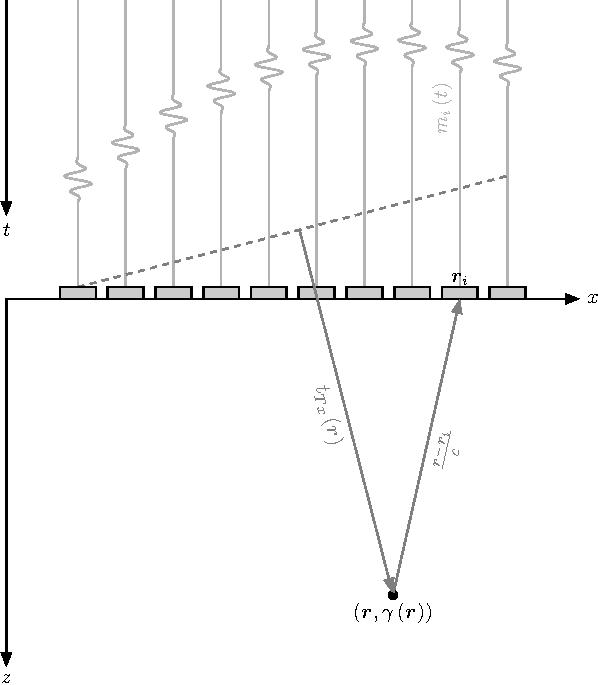
\includegraphics[width=0.9\linewidth]{tikz_SPARS-crop.pdf}
				\caption{Standard setting for US imaging}
			\end{figure}
		\end{column}
	\end{columns} % End of the subdivision
	
	\begin{itemize}
		\item The signals received at each element follow a \textbf{stream of pulses} model and can be written as:
		\begin{equation*}
		m_i\left(t\right)~=~\sum_{k=1}^{K} a_{ik} \psi \left(t - t_{k}\right)
		\end{equation*}
		with $\left(a_{ik}, t_{k}\right)_{k=1}^K$ amplitudes and times-of-arrival of the $K$ echo-pulses to the $i^{th}$ transducer-element
		\item The $N_t$ discretized samples obtained by sampling $m_i\left(t\right)$ at a frequency $f_s$ \textbf{obey a $K$-sparse synthesis model} in a dictionary $\Psi \in \mathbb{R}^{N_t \times N_t}$ made of all the shifted replicas of the pulse~\cite{naini2009}:
		\begin{equation*}
			\bm{m}_i = \Psi \bm{a}_i, \textnormal{ with } \| \bm{a}_i\|_0 = K
		\end{equation*}
	\end{itemize}
	
\end{block}
\vfill 
%----------------------------------------------------------------------------------------
%	METHODS
%----------------------------------------------------------------------------------------

\begin{block}{The proposed acquisition scheme: US compressive multiplexer}
	\begin{column}{.54\textwidth} % The first subdivided column within the first main column
		\begin{itemize}
			\item \textbf{CMUX}~\cite{kim2012}: Signals from M sensors are modulated and summed:
			\begin{equation*}
			y \left(t\right)~=~ \sum_{i=1}^{M} p_i \left(t\right) m_i \left(t\right)
			\end{equation*}
			where $p_i\left(t\right)$ is a chipping sequence drawn from a Rademacher distribution
			\item Signal $y \left(t\right)$ sampled at $f_s$ leading to a compression by a factor of M
			\item \textbf{US-CMUX}: Use L CMUX each of which grouping M sensors and sharing the same chipping sequences to perform signal acquisition
			\begin{equation*}
				\mathsf{Y} = \left[\bm{y_1}, ..., \bm{y_L}\right] \in \mathbb{R}^{N_t \times L}
			\end{equation*}
			\item Compression by a factor of M compared to standard US devices
			\item Can be achieved using mixed signal blocks~\cite{kim2012}
		\end{itemize}
	\end{column}
	\begin{column}{.43\textwidth}
		\begin{figure}[htb]
			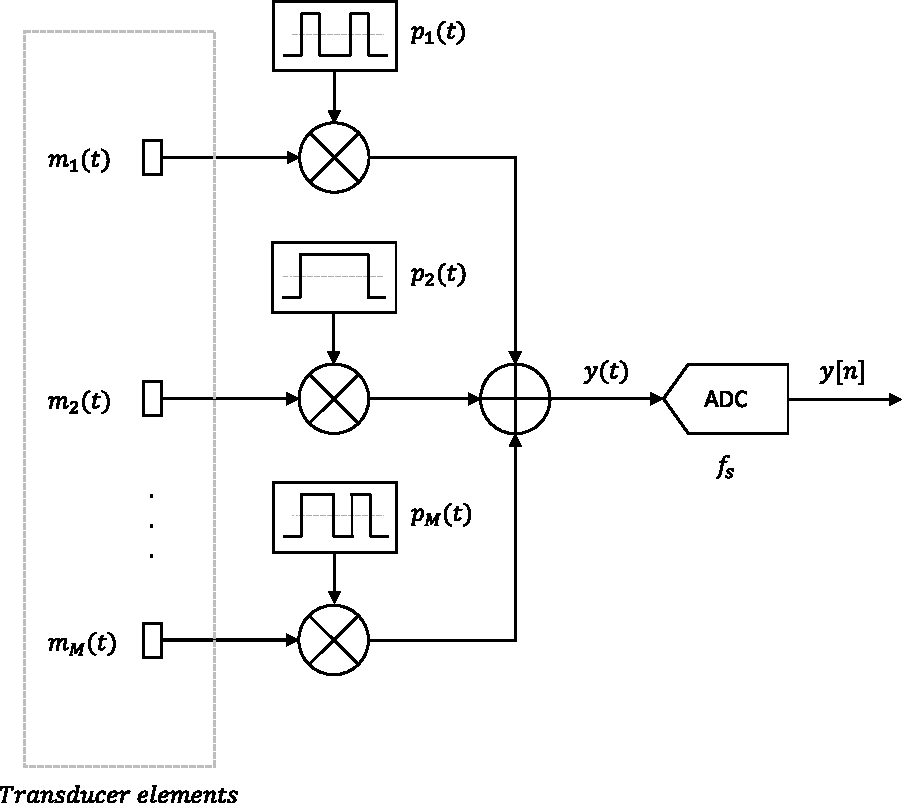
\includegraphics[width=0.8\linewidth]{figures/CMUX.pdf}
			\caption{CMUX architecture}
			\label{fig_CMUX}
		\end{figure}
	\begin{figure}[htb]
		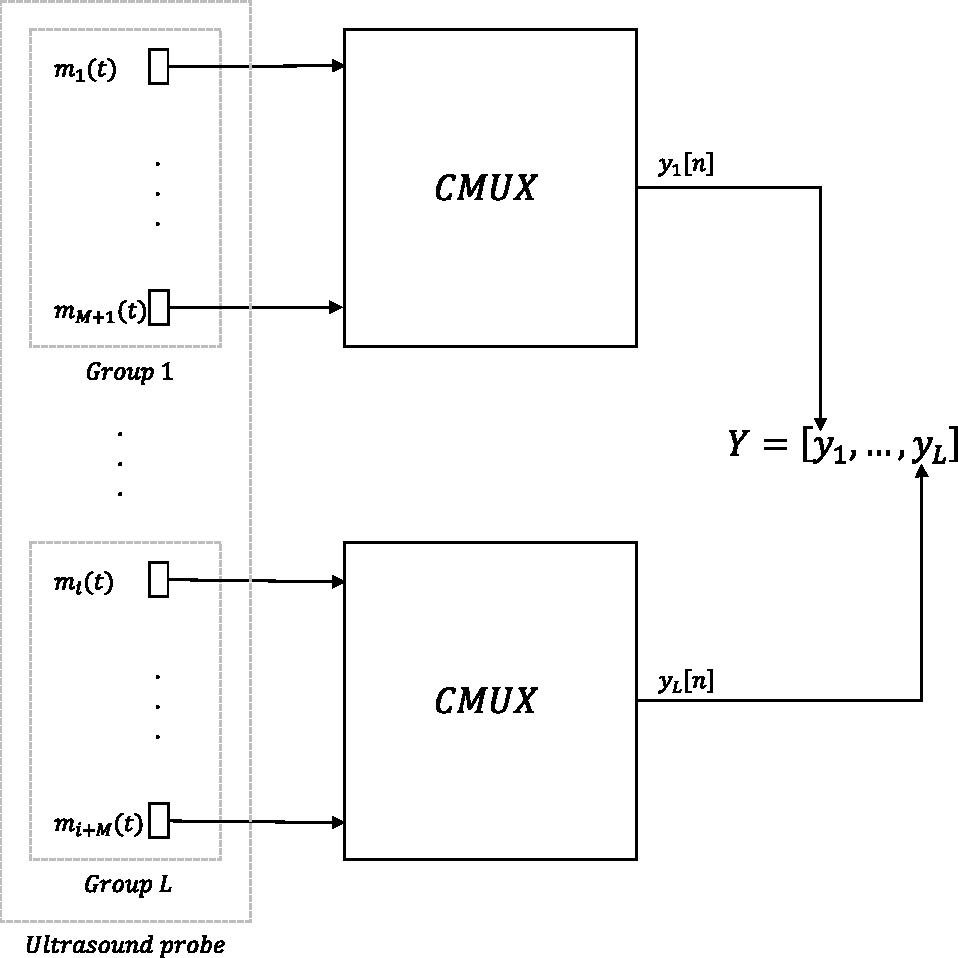
\includegraphics[width=0.8\linewidth]{figures/USCMUX.pdf}
		\caption{US-CMUX architecture}
		\label{fig_USCMUX}
	\end{figure}
	\end{column}
	
\end{block}
\vfill
%----------------------------------------------------------------------------------------
%	US image reconstruction
%----------------------------------------------------------------------------------------

\begin{block}{Proposed reconstruction algorithm}
	\begin{itemize}
		\item $\ell_{11}$-minimization problem is solved:
		\begin{equation*}
		\min_{\bar{\mathsf{A}} \in \mathbb{R}^{MN_t \times L}} \lVert \bar{\mathsf{A}} \lVert_{11}
		\textnormal{ subject to } \| \mathsf{Y}- \Psi_{P}\bar{\mathsf{A}}\|_F\leq\epsilon
		\end{equation*}
		$\Psi_{P}~=~\left[\Psi_{p1}, ..., \Psi_{pM}\right] \in \mathbb{R}^{N_t \times M N_t}$, $\Psi_{pi}~=~\left[\bm{p}_i \otimes \Psi_1, ..., \bm{p}_i \otimes \Psi_{N_t}\right] \in \mathbb{R}^{N_t \times N_t}$ 
		\begin{equation*}
		\mathsf{A}=
		\begin{bmatrix}
		\bm{a}_1 & \bm{a}_{M+1} & \dotsb & \bm{a}_{N_{el}-M+1}\\
		\vdots & \vdots & & \vdots \\
		\bm{a}_M & \bm{a}_{2M} & \dotsb &\bm{a}_{N_{el}} \\
		\end{bmatrix}
		\end{equation*}
		\item Solved with primal dual forward backward algorithm~\cite{combettes2014} 
	\end{itemize}
\end{block}
%----------------------------------------------------------------------------------------
}%
			\end{column} % End of the first column
	
			\AddBlankColumn % Empty spacer column
	
			\begin{column}{\RightColumnWidth} % The second column
				\vbox to \myposterheight{%
\begin{block}{Experimental setup}
	\begin{itemize}
		\item Data acquisition:
		\begin{itemize}
			\item \textit{In-vitro} hyperechoic inclusion phantom~(Model 54GS, CIRS Inc., Norfolk, USA) and \textit{in-vivo} carotids
			\item Data acquired with a Verasonics research scanner~(V1-128, Verasonics Inc., Redmond, WA)
			\item ATL L12-5~\SI{50}{\milli\metre} ultrasound probe used for the different experiments
			\begin{itemize}
				\item \num{128} active transducer-elements
				\item \SI{5}{\mega\hertz} central frequency with \SI{100}{\percent} bandwidth
				\item \SI{31.2}{\mega\hertz} sampling frequency
			\end{itemize} 
			\item Transmission of plane waves with normal incidence
		\end{itemize}
		\item US-CMUX architecture 
		\begin{itemize}
			\item Simulated on MATLAB\textsuperscript{\textregistered}
			\item \num{2} cases: L=2 and L=4 
			\item Parameters of the reconstruction algorithm: $\epsilon = 10^{-6} \| \mathsf{Y}\|_F$, \num{1500} iterations
		\end{itemize}
		\item Image reconstruction:
		\begin{itemize}
			\item Achieved with standard delay-and-sum algorithm
			\item Post-processing pipeline for B-mode image
			\begin{itemize}
				\item Envelope extraction: Hilbert transform
				\item Normalization and log-compression with a dynamic range of \SI{40}{\decibel} 
			\end{itemize}
		\end{itemize}
	\end{itemize}
\end{block}
\vfill
%----------------------------------------------------------------------------------------
%	RECONSTRUCTED IMAGES
%----------------------------------------------------------------------------------------

\begin{block}{Reconstructed B-mode images}
	
	\newlength{\CIRSFigWidth} \setlength{\CIRSFigWidth}{0.24\textwidth}
	\newlength{\CIRSFigHeight}
	\settoheight{\CIRSFigHeight}{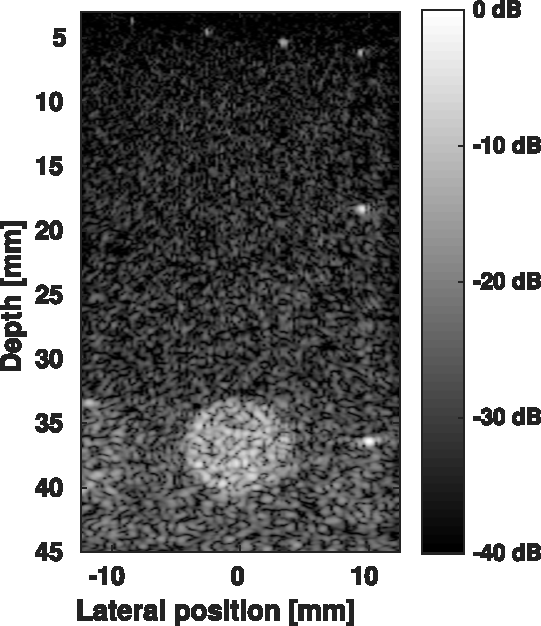
\includegraphics[width=\CIRSFigWidth]{figures/CS_hyperechoic.pdf}}
	\newlength{\CarotidFigWidth} \setlength{\CarotidFigWidth}{0.24\textwidth}
	\newlength{\CarotidFigHeight}
	\settoheight{\CarotidFigHeight}{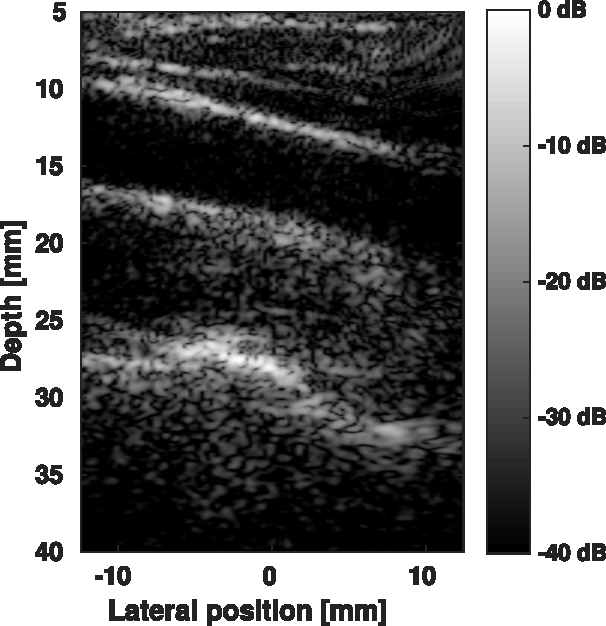
\includegraphics[width=\CarotidFigWidth]{figures/Reference_carotid.pdf}}  
	\begin{figure}
		\centering
		% Maximum length
		\subcaptionbox{Reference }{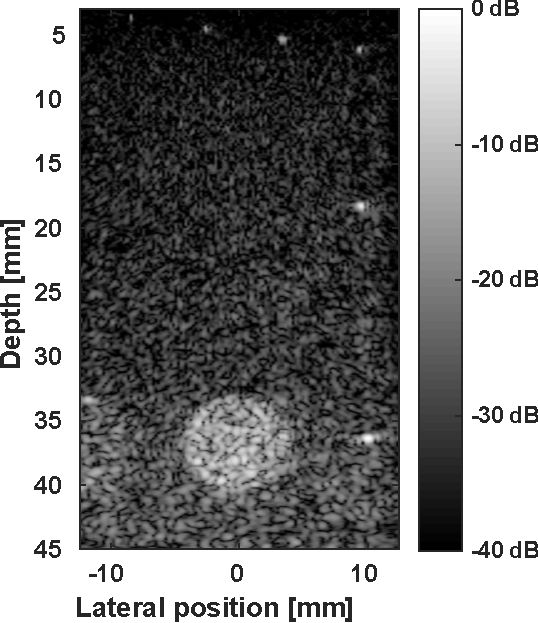
\includegraphics[height=\CIRSFigHeight]{figures/Reference_hyperechoic.pdf}}
		\subcaptionbox{CS reconstruction }{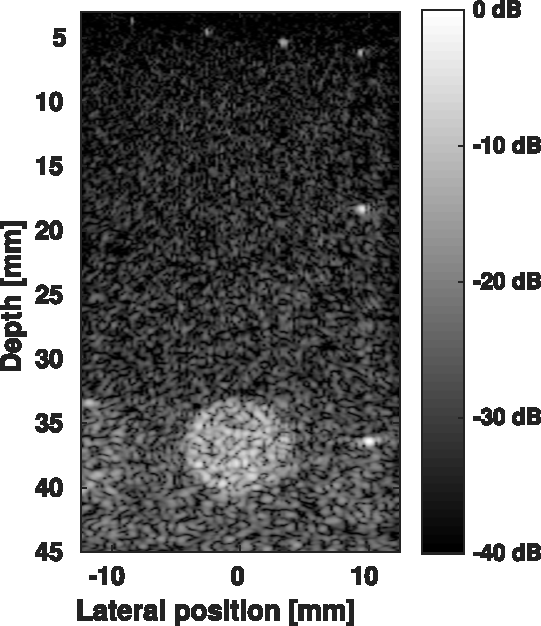
\includegraphics[height=\CIRSFigHeight]{figures/CS_hyperechoic.pdf}}
		\subcaptionbox{Reference }{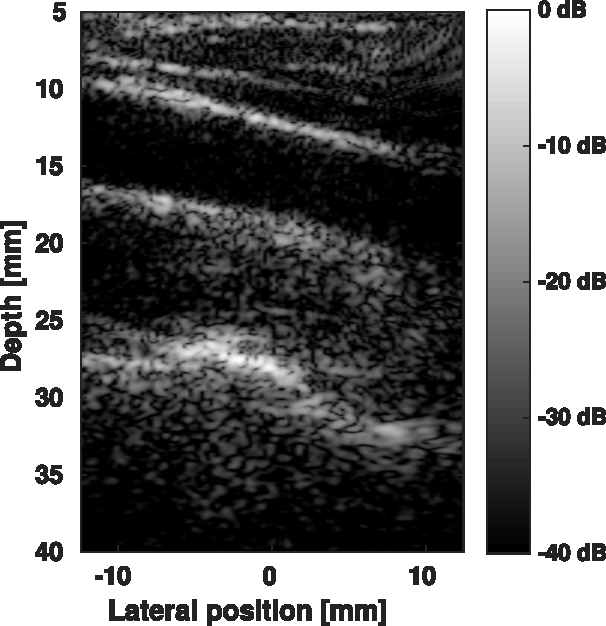
\includegraphics[height=\CarotidFigHeight]{figures/Reference_carotid.pdf}}
		\subcaptionbox{CS reconstruction }{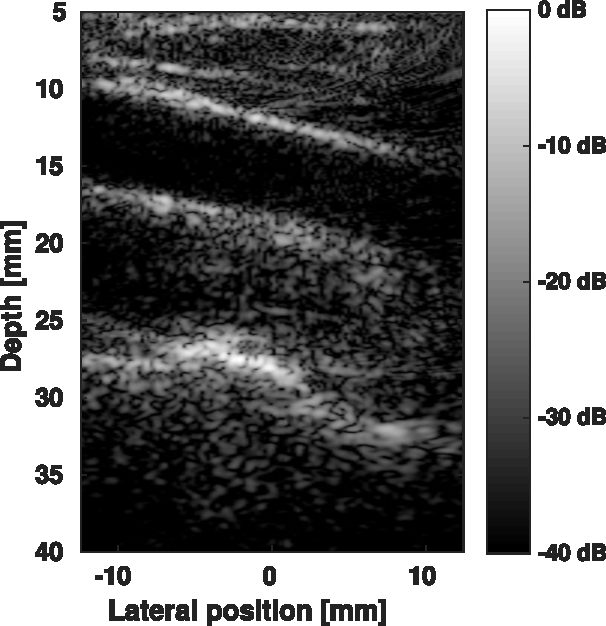
\includegraphics[height=\CarotidFigHeight]{figures/CS_carotid.pdf}}
		\caption{B-mode images of the hyperechoic inclusion and the carotid reconstructed with \SI{100}{\percent} of the data~((a) and (c)) and with \SI{25}{\percent} of the data acquired with US-CMUX~((b) and (d))}
	\end{figure}
	
\end{block}
\vfill
%----------------------------------------------------------------------------------------
%	IMAGE QUALITY METRICS
%----------------------------------------------------------------------------------------
\begin{block}{Quality metrics of the reconstructed images}
	\begin{itemize}
		\item PSNR and SSIM against B-mode images reconstructed with \SI{100}{\percent} data
	\begin{table}[htb]
		\caption{Average PSNR~$\left[\si{\decibel}\right]$ and SSIM~$\left[-\right]$ over \num{10} draws for the different images}
		\label{tab:SNR_SSIM}
		\centering
		\begin{tabular}{|c |c c|}
			\hline
			& Hyperechoic inclusion & \textit{In-vivo} carotid\\
			\hline
			PSNR - $L = 2$ & $39$ & $36$\\
			SSIM - $L = 2$ & $0.94$ & $0.87$\\
			PSNR - $L = 4$ & $32$ & $29$ \\
			SSIM - $L = 4$ & $0.81$ & $0.72$\\
			\hline
		\end{tabular}
	\end{table} 
		\item High quality reconstruction with \SI{25}{\percent} of the data.
	\end{itemize}
\end{block}
\vfill
%----------------------------------------------------------------------------------------
%	CONCLUSION
%----------------------------------------------------------------------------------------
\begin{block}{Conclusion and perspectives}
	\begin{enumerate}
		\item We propose a compressed sensing approach for US image recovery
		\begin{itemize}
			\item Exploits a stream of pulses model for sparsity of US images
			\item Uses multiple CMUX for analog compression of the data
			\item Applies a $\ell_{11}$-minimization algorithm for image reconstruction
		\end{itemize}
		\item The proposed approach leads to high-quality reconstruction with far fewer data than standard approaches
		\item Study of the hardware implementation will be achieved in future work
	\end{enumerate}
\end{block}
\vfill
%----------------------------------------------------------------------------------------
%	BIBLIOGRAPHY
%----------------------------------------------------------------------------------------
\begin{block}{References}
	\printbibliography
\end{block}
\vfill
%----------------------------------------------------------------------------------------
%	ACKNOWLEDGMENTS
%----------------------------------------------------------------------------------------
\begin{block}{Acknowledgments}
	This work was supported in part by the UltrasoundToGo RTD project (no. 20NA21 145911), evaluated by the Swiss NSF and funded by Nano-Tera.ch with Swiss Confederation financing.The authors would like to thank Dr~Olivier Bernard from CREATIS laboratory for providing the \textit{in vitro} and \textit{in vivo} acquisition data.
\end{block}
}%
			\end{column} % End of the second column
	
			\AddBlankColumn % Empty spacer column
	
		\end{columns} % End of all the columns in the poster

	\end{frame} % End of the enclosing frame

\end{document}
